\documentclass[11pt,a4paper]{article}
\usepackage[latin1]{inputenc}
\usepackage[english]{babel}
\usepackage{amsmath}
\usepackage{amsfonts}
\usepackage{amssymb}
\usepackage{graphicx}
\usepackage{grffile}
\usepackage[left=2cm,right=2cm,top=2cm,bottom=2cm]{geometry}
\author{Tobias Stål}
\begin{document}


This document is written in \LaTeX.

Here is a plot generated in matplotlib from the script result1.py:

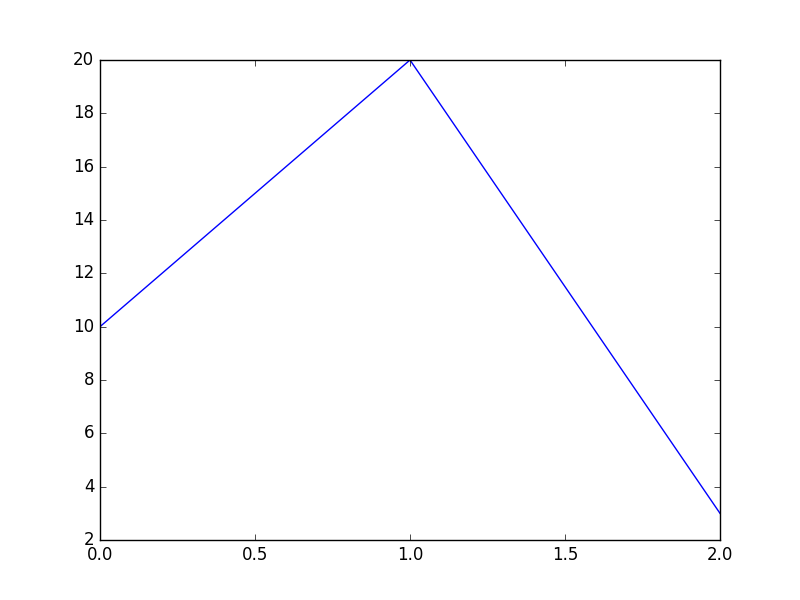
\includegraphics[scale=0.5]{fig/plot1.png}

Here is a more complex plot, also generated from matplotlib. 

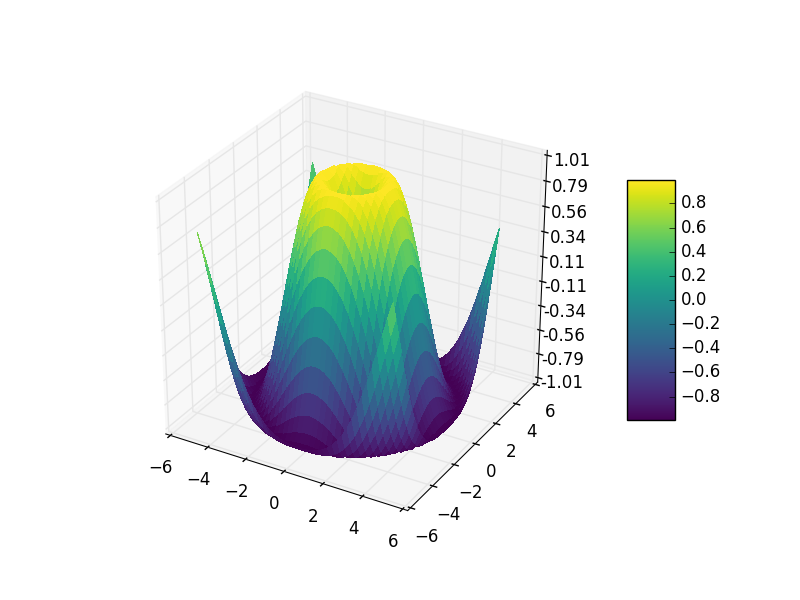
\includegraphics[scale=0.5]{fig/plot2.png}


Here is some more text, imported from a textfile generated by a python script. 

\input{txt/results1.txt}

An here is a map generated by a shellscript

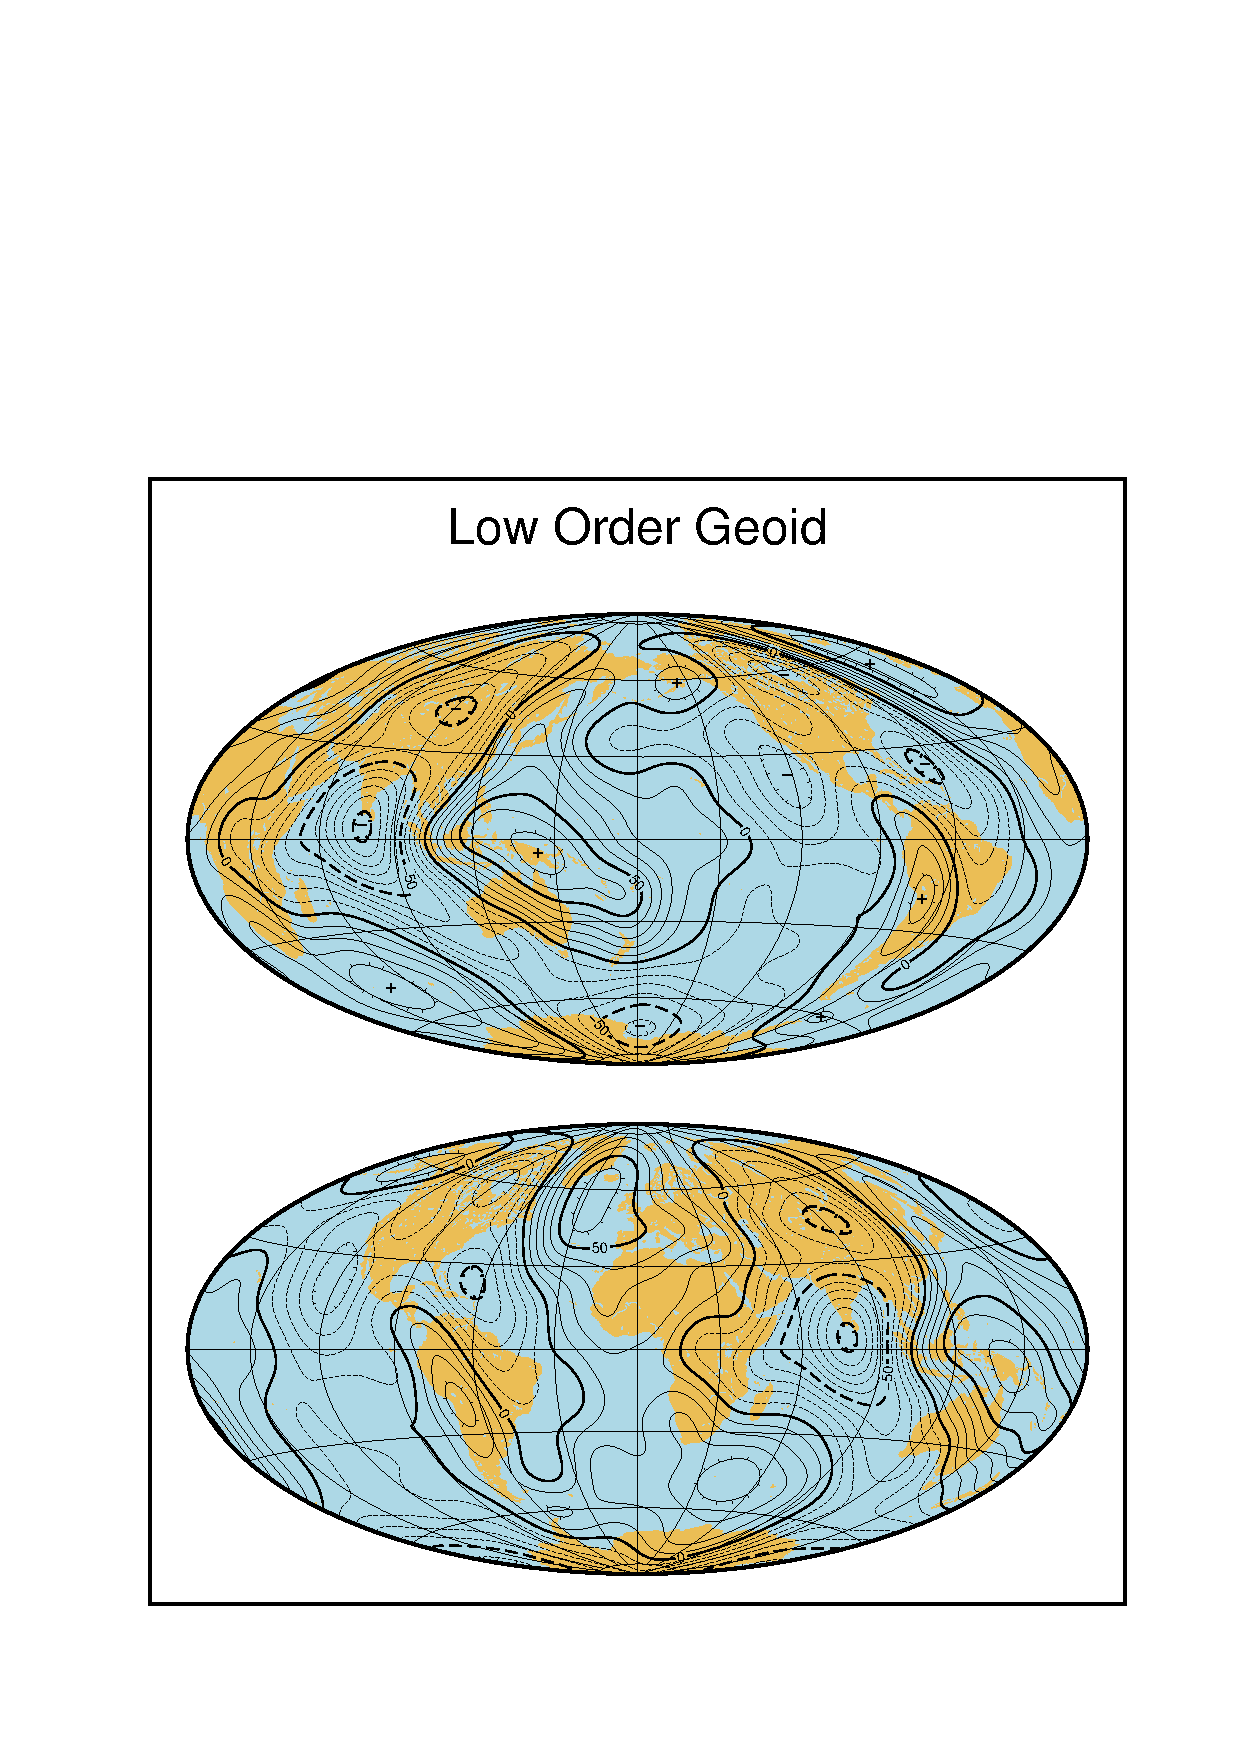
\includegraphics[scale=0.5]{fig/map1.pdf}

And here is a map generated directely by shell commands in the SConstruct file. 

%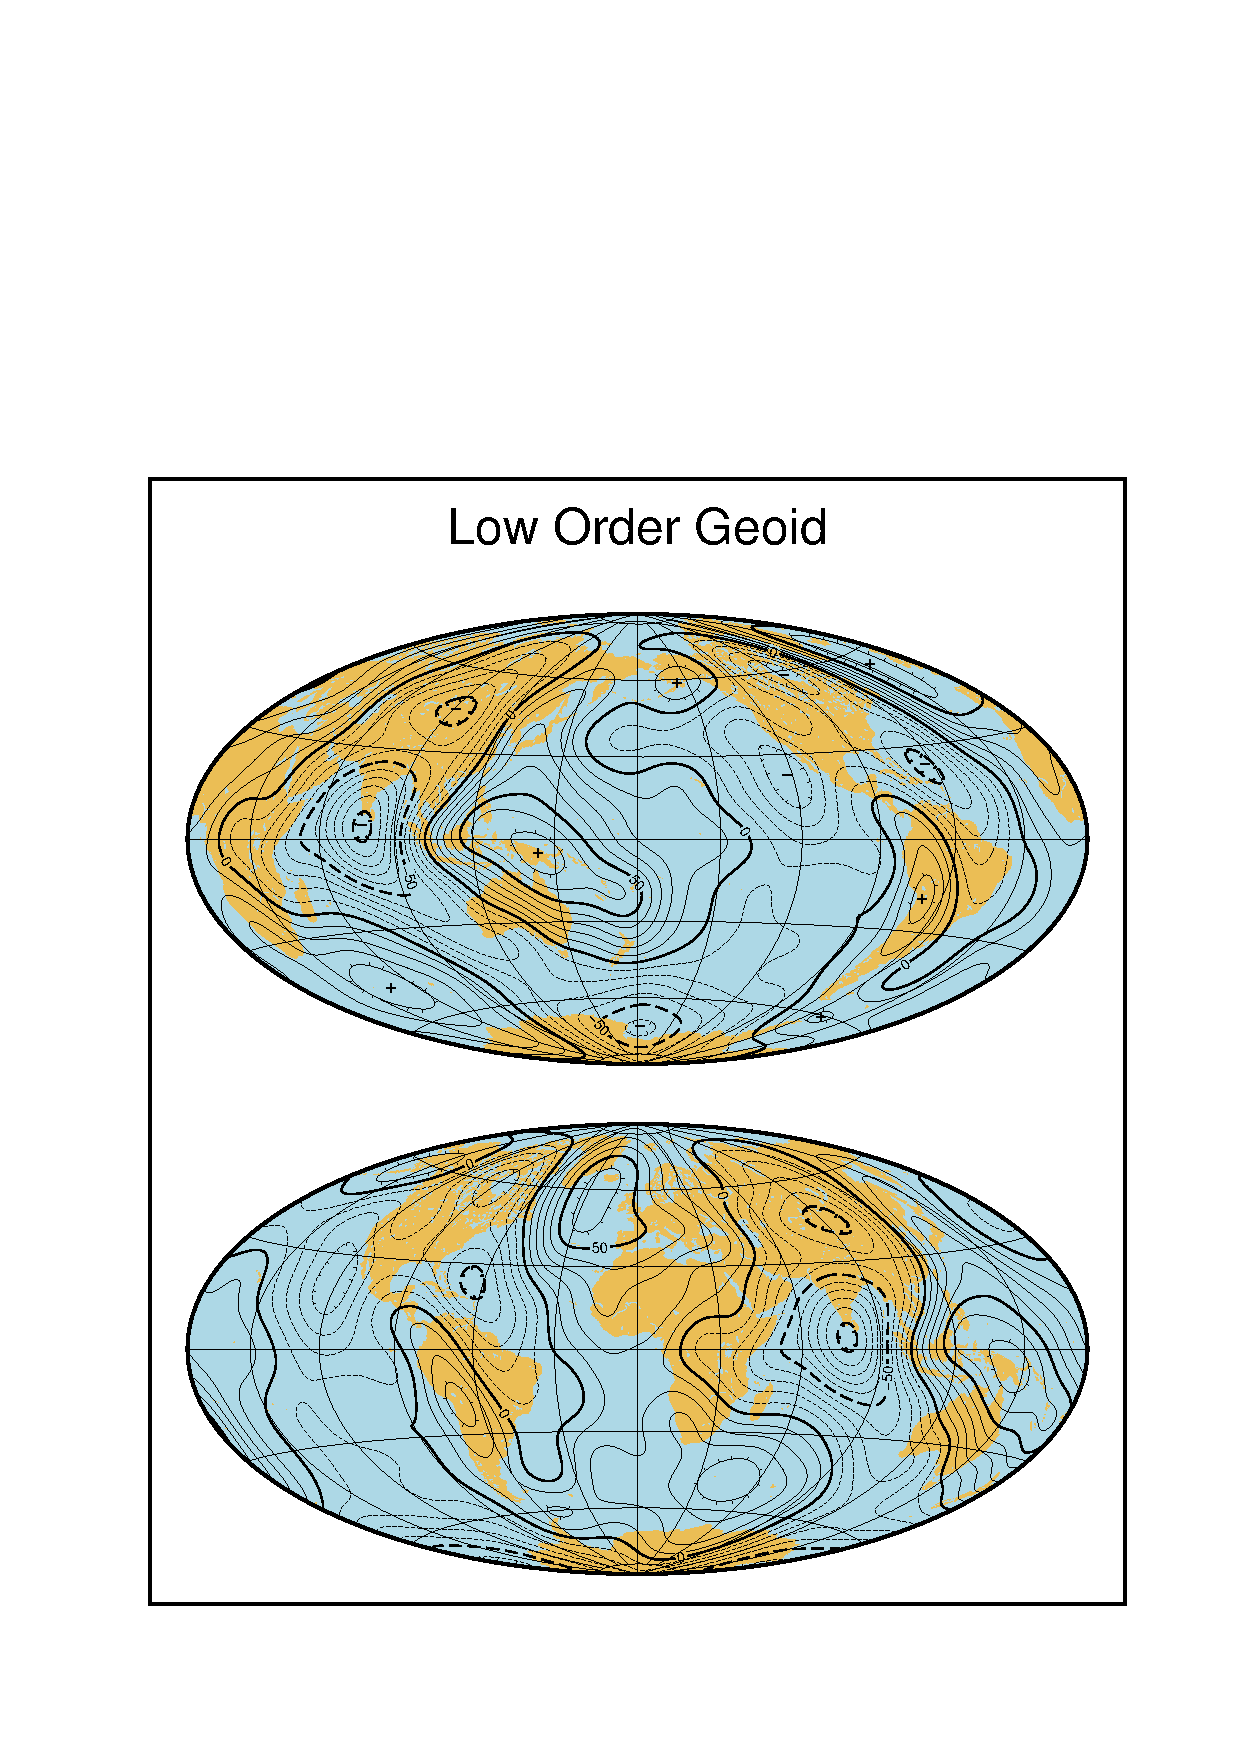
\includegraphics[scale=0.5]{fig/map1.pdf}

Here will be a tikZ illustration. 

And biography. 

And maybe a madagascar exemple. 


\end{document}